% =============================================================================
\documentclass[a0paper,portrait, blockverticalspace=3em, colspace=2em]{tikzposter}
\tikzposterlatexaffectionproofoff
\usepackage{graphicx}
\usepackage{amsmath}
\usepackage{amssymb}
\usepackage{multicol}
\usetikzlibrary{calc}

\newcommand{\looseitems}{\begin{itemize}\setlength{\itemsep}{0.3em}}
\newcommand{\tightitems}{\begin{itemize}\setlength{\itemsep}{0.15em}}
\newcommand{\captiontext}[1]{#1}

\usetheme{Default}

\title{\parbox{0.74\linewidth}{\centering\huge
    Irradiation Studies and Design Optimization of the ATLAS Tile Calorimeter for the High-Luminosity LHC\\[1mm]
    }}
\author{\Large Róbert Astalos (Comenius University Bratislava), on behalf of the ATLAS Tile Calorimeter System}
\institute{\normalsize International Workshops on Radiation Imaging Detectors, Ghent, 28.6.–02.07.2026}
\date{}

\begin{document}
\maketitle

\begin{columns}

  % ===== Column 1 =====
  \column{0.333}

    % block id: blk_tilecal  (column 1, order 0)
    \block{The ATLAS Hadronic Tile Calorimeter (TileCal)}{
      \begin{itemize}\setlength{\itemsep}{0.3em}
        \item The Tile Calorimeter is a hadronic calorimeter composed of wedge-shaped modules arranged in a Long Barrel (LB) and two Extended Barrels (EB).
        \item Consists of 256 modules containing 5182 calorimetric cells, utilizing scintillating tiles and wavelength shifting fibers to transfer light to photomultiplier tubes (PMTs). Most cells are readout by two PMTs, except for special E1–E4 gap/crack cells readout by one PMT.
        \item \textbf{Low Voltage Power Supplies (LVPS)}: Utilize switching DC-DC converters (bricks) at 300 kHz to step down a bulk 200 V input to different voltage levels to distribute stable power to the on-detector readout electronics.
        \item \textbf{Daughterboard (DB)}: central communication hub of each module, using high-speed optical links to continuously transmit digitized PMT signals to off-detector systems while receiving timing and configuration commands.
        \item Components located in the highest radiation regions of TileCal, particularly the LB LVPS and readout electronics close to the detector gap regions, must tolerate elevated TID and NIEL levels.
        \item Single Event Effects (SEE), in particular Single Event Upsets (SEU) and Single Event Latch-ups (SEL), must be evaluated and mitigated.
      \end{itemize}

      \begin{minipage}{0.495\linewidth}
        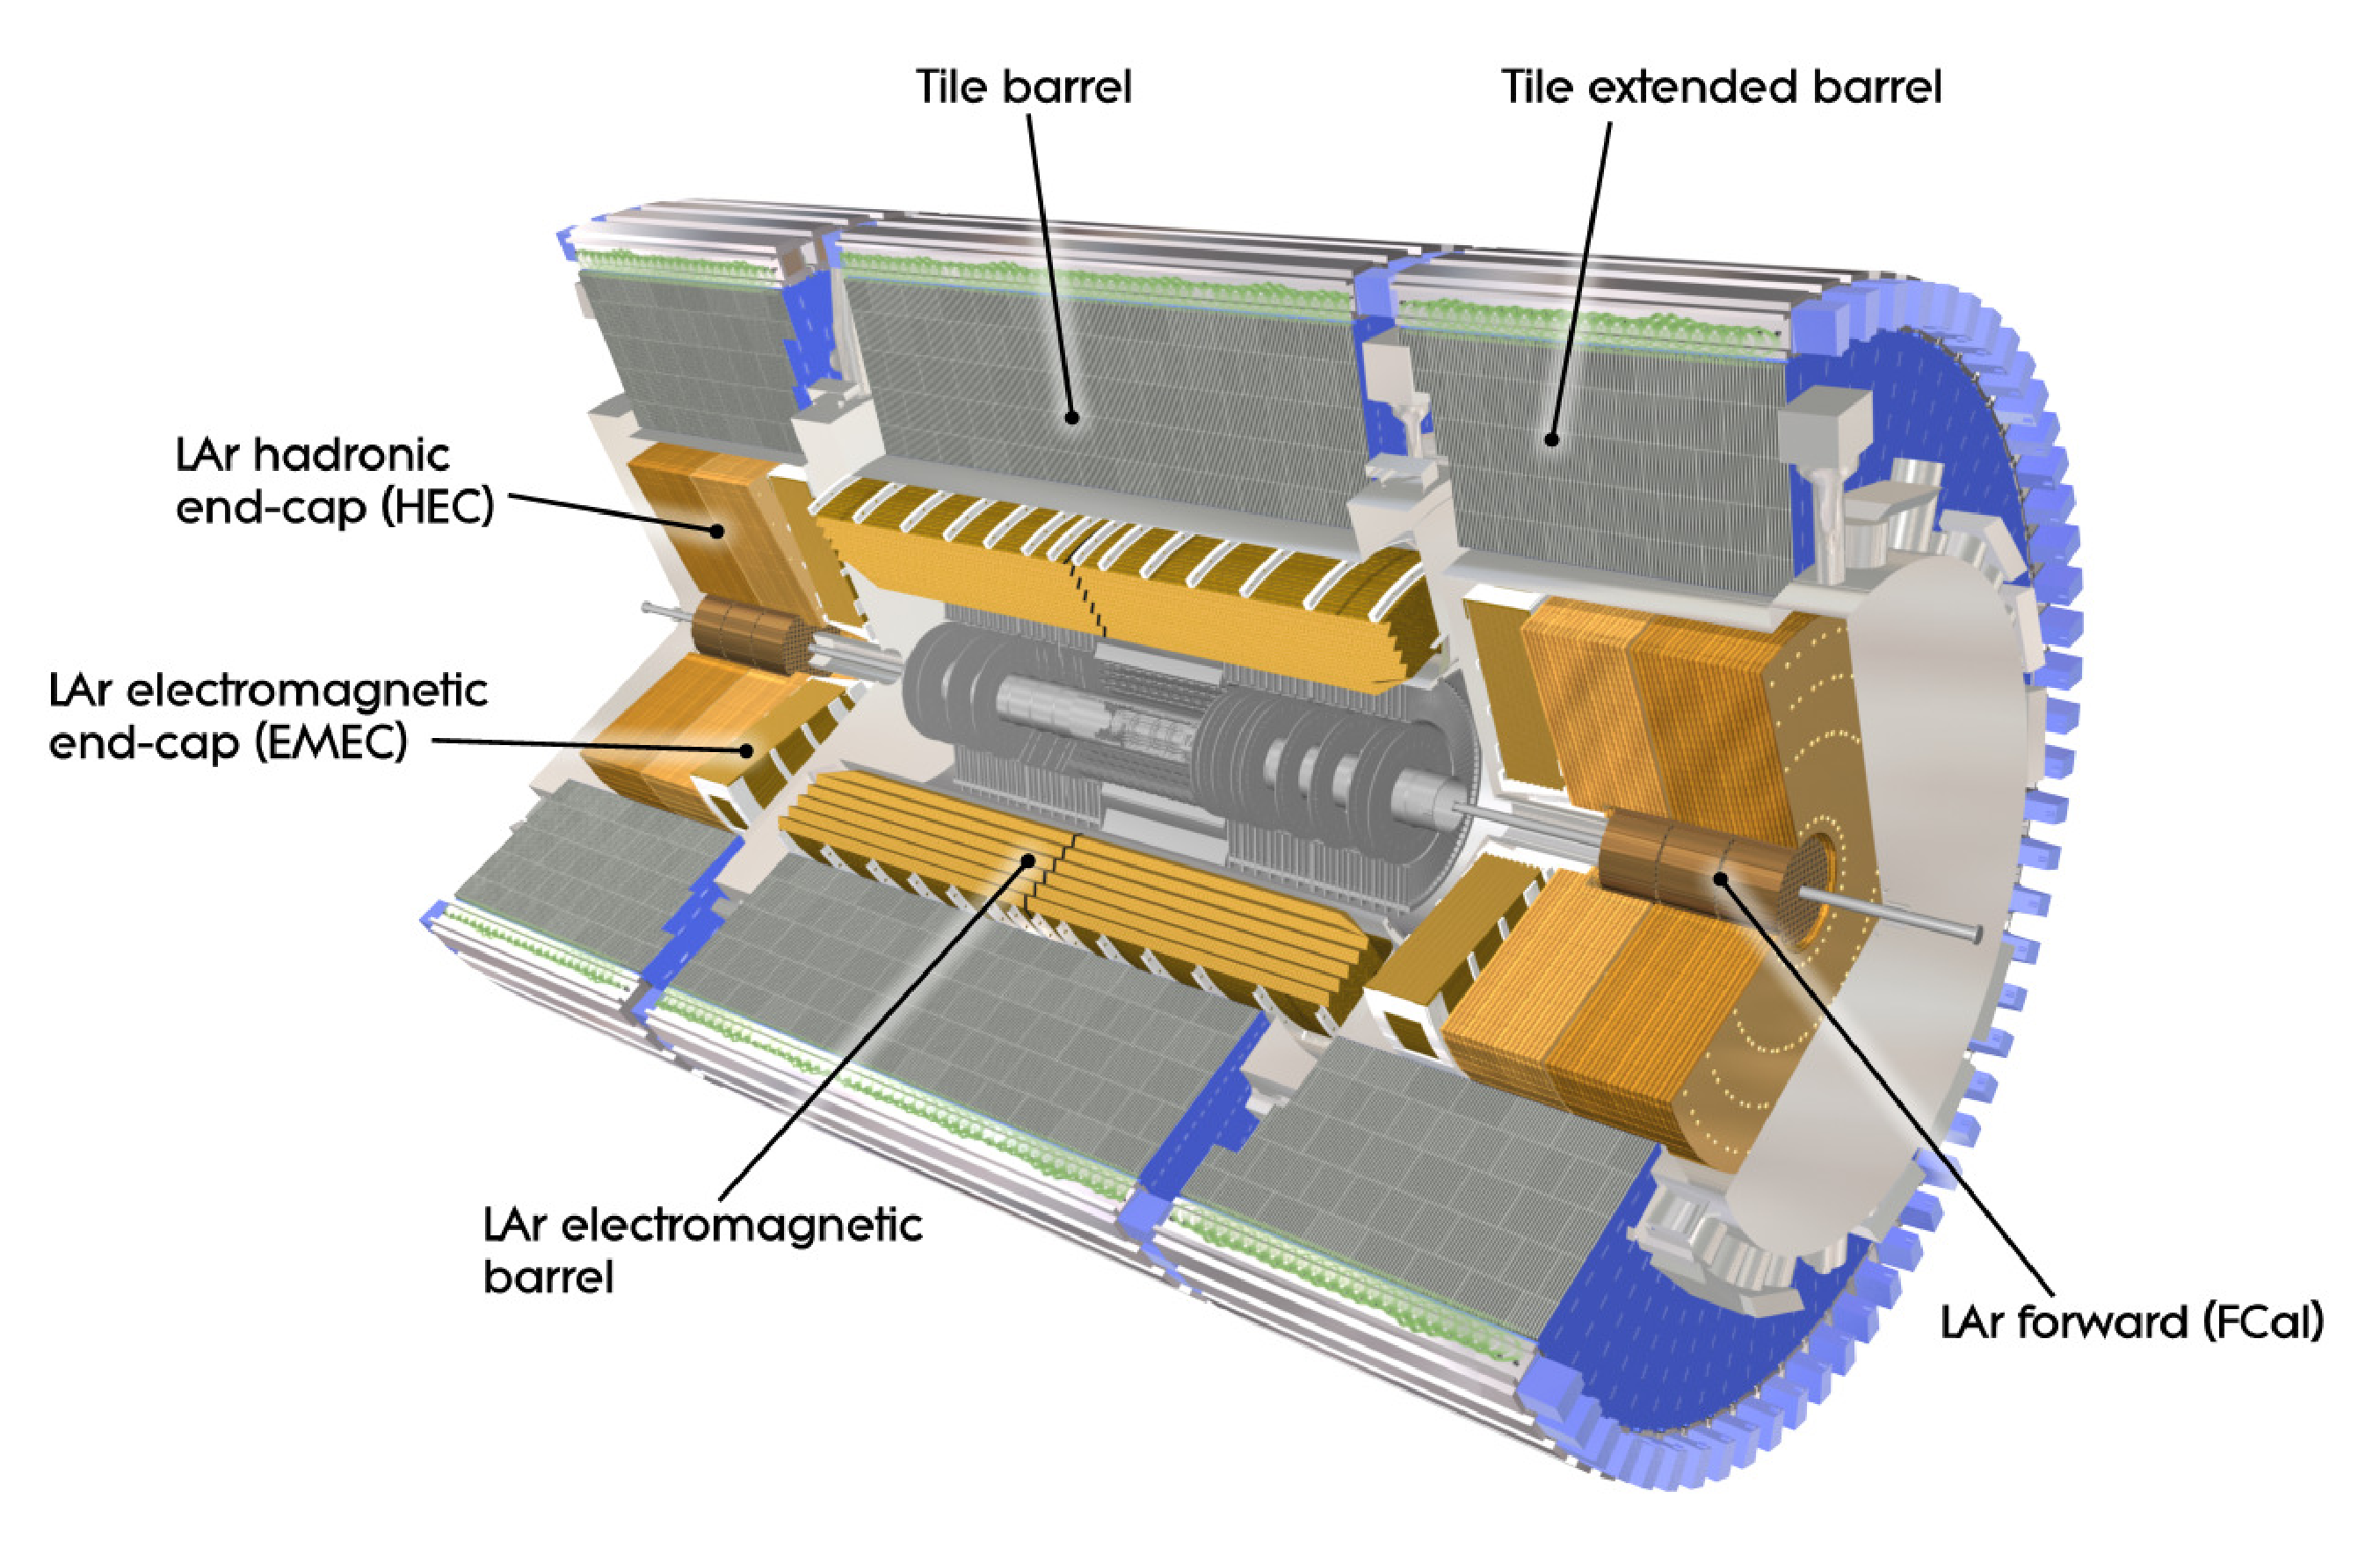
\includegraphics[width=\linewidth]{assets/plot1.pdf}
      \end{minipage}%
      \hfill
      \begin{minipage}{0.495\linewidth}
        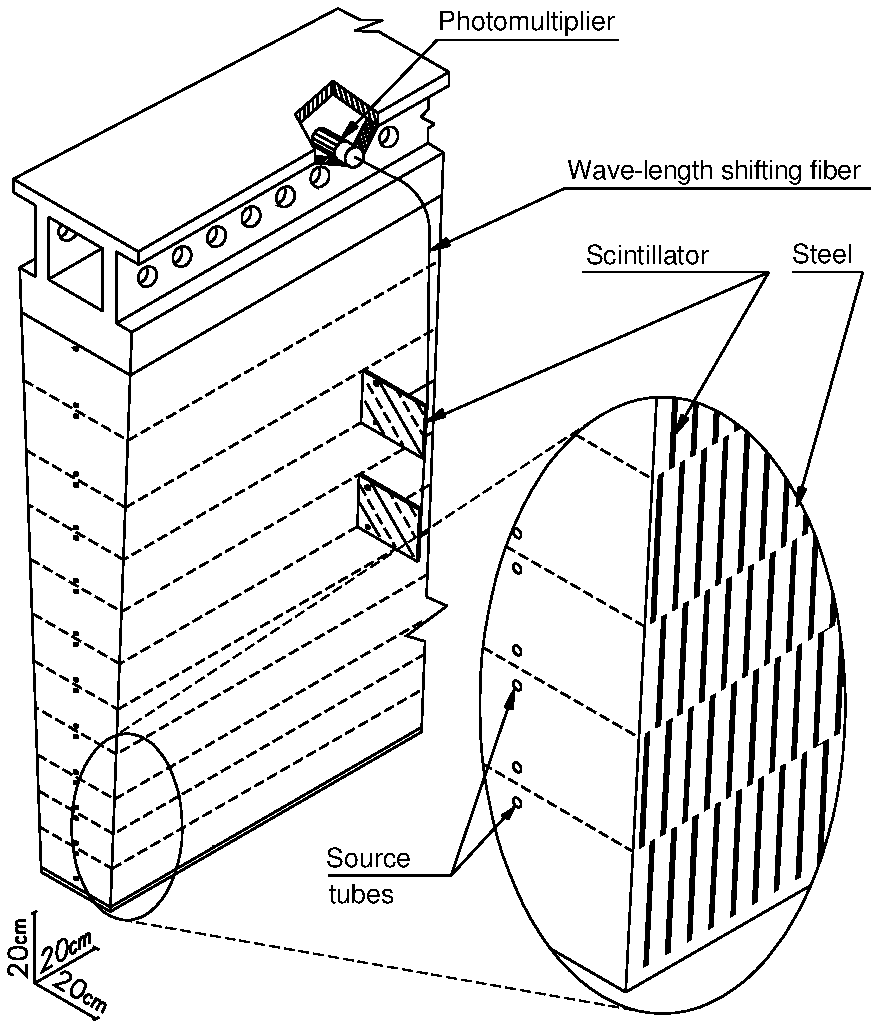
\includegraphics[width=\linewidth]{assets/plot2.pdf}
      \end{minipage}

        {\small Figure 1: ATLAS Tile Calorimeter (left) and a wedge-shaped module slice (right) [1].}
    }

    % block id: blk_radiation_criteria  (column 1, order 1)
    \block{Radiation Criteria}{
      \begin{itemize}\setlength{\itemsep}{0.3em}
        \item Simulated radiation criteria for the HL-LHC includes safety factors up to 5.0 for TID (low dose rate) and 2.0 for SEE.
      \end{itemize}

      \resizebox{\linewidth}{!}{
      \begin{tabular}{|l|c|c|c|}\hline
        \hline
        Component & TID [Gy] & NIEL [n/cm²] & SEE [p/cm²] \\
        \hline
        PMT Divider – Barrel & 17.6 & 2.0×10¹² & 1.9×10¹¹ \\
        FENICS – Barrel & 10.6 & 1.6×10¹² & 1.8×10¹¹ \\
        MB – Barrel & 10.0 & 1.4×10¹² & 9.2×10¹⁰ \\
        LVPS – Barrel & 53.6 & 3.5×10¹² & 5.3×10¹¹ \\
        DB – Endcap & 6.8 & 9.7×10¹¹ & 4.9×10¹⁰ \\
      \hline
      \end{tabular}
      }
      {\small Table 1: Simulated worst-case doses for 4000 fb⁻¹ (no safety factors), only higher doses from Barrel/Endcap are shown.}
    }

  % ===== Column 2 =====
  \column{0.333}

    % block id: blk_lvps  (column 2, order 0)
    \block{LVPS Design \& Component Radiation Testing}{
      \begin{itemize}\setlength{\itemsep}{0.3em}
        \item \textbf{LVPS Design:} 8 identical bricks for LB modules and 6 bricks for EB modules inside a box convert the 200 V input to a 10 V output at a nominal power of 23 W – Each brick powers an independent side of the readout electronics, preserving the TileCal dual-PMT cell redundancy.
        \item Replacing original STB57N65M5 power MOSFETs with SIHFS9N60A reduced gate-source capacitance and switching losses. Efficiency improved from 58\% to 72\%, meeting the 77 kW cooling capacity of the TileCal cooling system.
        \item Control interface optimization reduced the number of required control lines by 50\%, enabling reuse of the existing infrastructure. The optimization successfully achieved the project targets, ensuring operational stability and mitigating failure risks.
        \item \textbf{Radiation Testing:} SIHFS9N60A MOSFET (main high-power switching transistor): Shift of 2.5 V in gate-source threshold observed after 200 Gy of TID, with minimal deviation from NIEL.
        \item SI8920 Isolation Amplifier: Initial tests showed voltage fluctuations at 150 mV, but performance is completely stable below 100 mV. Selected for final production with circuits restricting the input voltage.
        \item LT1681 Controller \& LT3080 Regulator: TID tests at 502 Gy/h showed minor drifts (≤5\%) in output voltages, within acceptable limits.
        \item LTC6241 Op-Amp: Single Event Transients (SETs) had small amplitudes (\textasciitilde{}50 mV) and short durations (\textasciitilde{}100 ns) posing no effect on brick performance.
      \end{itemize}

      \begin{minipage}{0.495\linewidth}
        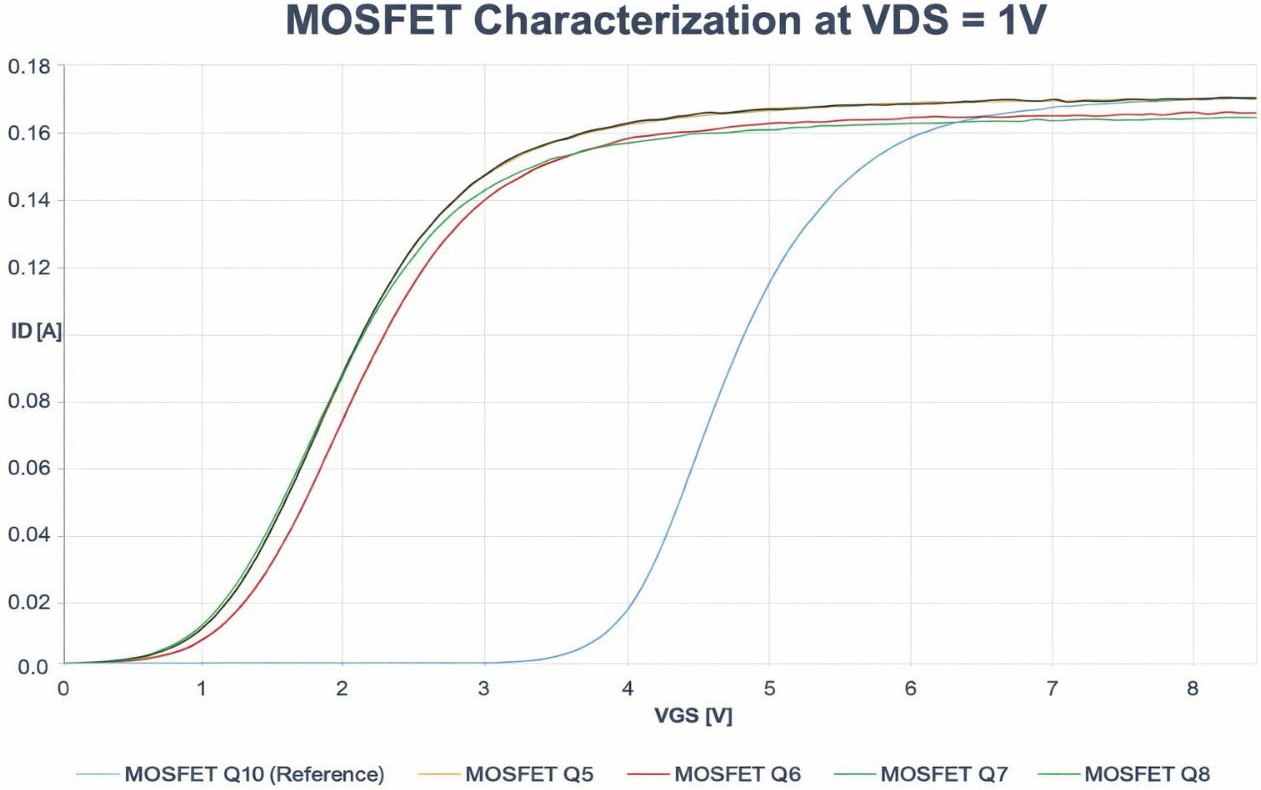
\includegraphics[width=\linewidth]{assets/Moayedi_2026_J._Inst._21_C05002_slide_7_item_1.png}
      \end{minipage}%
      \hfill
      \begin{minipage}{0.495\linewidth}
        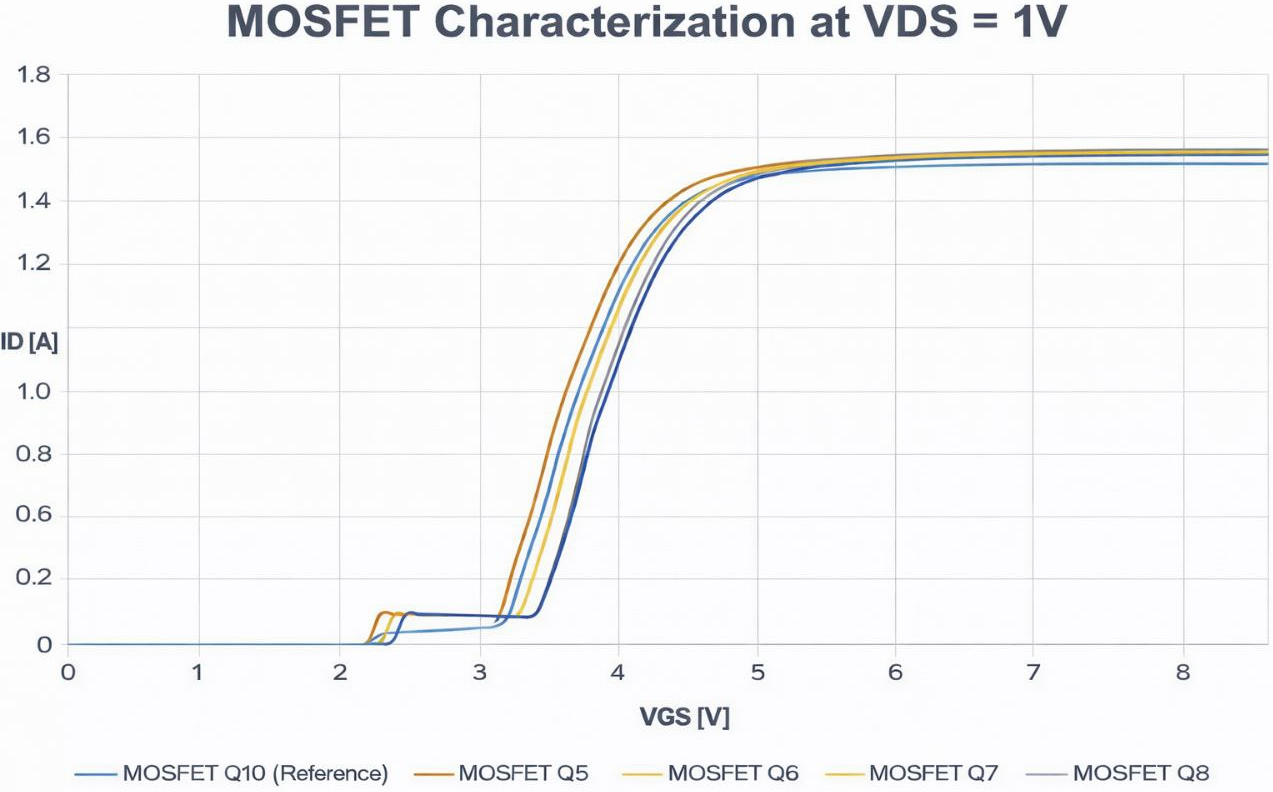
\includegraphics[width=\linewidth]{assets/Moayedi_2026_J._Inst._21_C05002_slide_7_item_2.png}
      \end{minipage}

        {\small Figure 2: SIHFS9N60A MOSFET characterization at V\_DS = 1 V after 200 Gy of TID (left) and after NIEL tests (right) [3].}
    }

  % ===== Column 3 =====
  \column{0.333}

    % block id: blk_db_architecture  (column 3, order 0)
    \block{Daughterboard (DB) Architecture}{
      \begin{itemize}\setlength{\itemsep}{0.3em}
        \item Interfaces the on-detector and off-detector systems by distributing timing and configuration signals and continuously transmitting digitized PMT data off-detector.
        \item 896 DBs will transmit \textasciitilde{}35 Tbps of physics data via 3584 optical uplinks (9.6 Gbps), while receiving configuration and timing via 1792 downlinks (4.8 Gbps).
        \item Utilizes Commercial Off-The-Shelf components and radiation-hard GBTx ASICs (receive clock and config commands) designed by CERN.
      \end{itemize}

      \begin{center}
        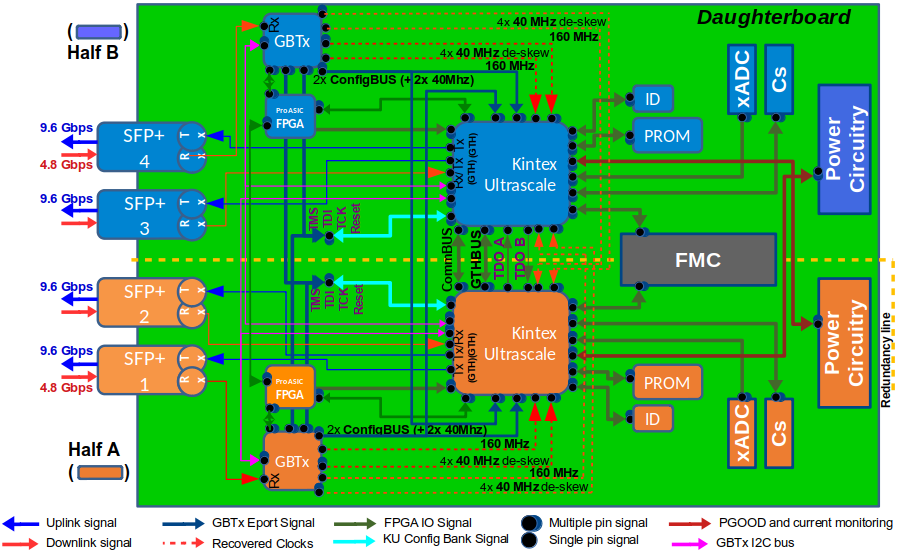
\includegraphics[width=1.0\linewidth]{assets/fig_db6_blockdiagram.png}
      \end{center}
      {\small Figure 3: The TileCal Daughterboard redundancy architecture and data paths [5].}
    }

    % block id: blk_db_qualification  (column 3, order 1)
    \block{DB Radiation Qualification \& Tolerances}{
      \begin{itemize}\setlength{\itemsep}{0.3em}
        \item The DB requires 108 Gy TID and 13.16×10¹² n/cm² NIEL qualification limits (including safety factors).
        \item Kintex Ultrascale (KU) FPGAs (primary data processors) and ProASIC FPGAs (remote reconfiguration buffers) successfully withstood over 108 Gy and 14×10¹² n/cm² during tests.
        \item KU+ FPGAs were disqualified for exhibiting SEL; selected KU FPGAs showed no SEL up to 3.2×10¹¹ p/cm².
        \item Measured SEU rates for the KU FPGA were 116 SEU/(10⁹ p/cm²); \textasciitilde{}5498 SEUs per year, heavily mitigated by Xilinx SEM.
      \end{itemize}

      \begin{center}
        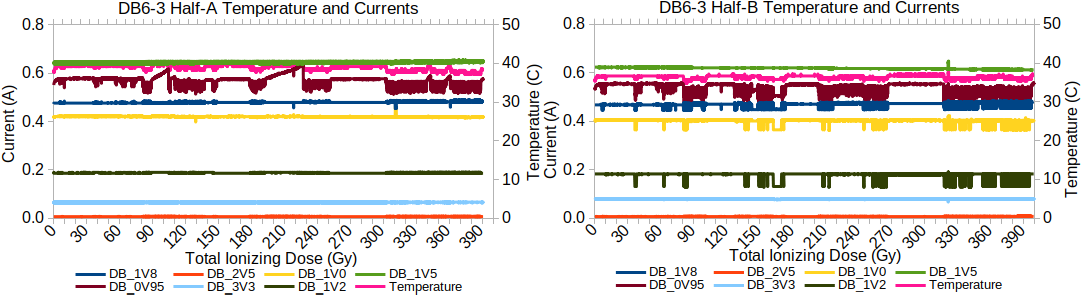
\includegraphics[width=1.0\linewidth]{assets/fig_db6_tid_test.png}
      \end{center}
      {\small Figure 4: Monitored KU FPGA temperatures and currents during 54 MeV proton beam TID testing. Drops correspond to active SEU corrections by the Xilinx SEM and resets applied during uncorrectable SEUs [5].}
    }

    % block id: blk_conclusions  (column 3, order 2)
    \block{Conclusions}{
      \begin{itemize}\setlength{\itemsep}{0.3em}
        \item The optimized power distribution scheme increases readout reliability, power efficiency, and mitigates failure impact by utilizing identical and independent LVPS bricks.
        \item DB key components passed TID and NIEL qualification, and SEL was eliminated from the selected KU FPGAs.
        \item All critical components for the upgrade of the TileCal on-detector electronics have been successfully qualified against the expected radiation environment, following all the safety factors imposed by CERN guidelines, enabling full-scale production.
      \end{itemize}
    }

    % block id: blk_references  (column 3, order 3)
    \block{References}{
      \begin{itemize}\setlength{\itemsep}{0.3em}
        \item ATLAS Collaboration, \textit{The ATLAS Experiment at the CERN Large Hadron Collider}, JINST 3 (2008) S08003.
        \item ATLAS collaboration, \textit{Technical Design Report for the Phase-II Upgrade of the ATLAS Tile Calorimeter}, CERN-LHCC-2017-019.
        \item S. Moayedi, \textit{Upgrade of the ATLAS Tile Calorimeter front-end power supply for the HL-LHC}, 2026 JINST \textbf{21} C05002.
        \item S. Moayedi, \textit{Upgrade of the ATLAS Tile Calorimeter Front-End Power Supply for the HL-LHC}, ATL-TILECAL-SLIDE-2025-552.
        \item E. Valdés Santurio et al., \textit{Radiation studies performed on the High Luminosity ATLAS TileCal link Daughterboard}, 2023 JINST \textbf{18} C04011.
      \end{itemize}
    }

\end{columns}
\end{document}